\documentclass[a4paper,12pt]{article}
%%%%%%%%%%%%%%%%%%%%%%%%%%%%%%%%%%%%%%%%%%%%%%%%%%%%%%%%%%%%%%%%%%%%%%%%%%%%%%%%%%%%%%%%%%%%%%%%%%%%%%%%%%%%%%%%%%%%%%%%%%%%%%%%%%%%%%%%%%%%%%%%%%%%%%%%%%%%%%%%%%%%%%%%%%%%%%%%%%%%%%%%%%%%%%%%%%%%%%%%%%%%%%%%%%%%%%%%%%%%%%%%%%%%%%%%%%%%%%%%%%%%%%%%%%%%
\usepackage{eurosym}
\usepackage{vmargin}
\usepackage{amsmath}
\usepackage{graphics}
\usepackage{framed}
\usepackage{epsfig}
\usepackage{subfigure}
\usepackage{fancyhdr}

\setcounter{MaxMatrixCols}{10}
%TCIDATA{OutputFilter=LATEX.DLL}
%TCIDATA{Version=5.00.0.2570}
%TCIDATA{<META NAME="SaveForMode"CONTENT="1">}
%TCIDATA{LastRevised=Wednesday, February 23, 201113:24:34}
%TCIDATA{<META NAME="GraphicsSave" CONTENT="32">}
%TCIDATA{Language=American English}

\pagestyle{fancy}
\setmarginsrb{20mm}{0mm}{20mm}{25mm}{12mm}{11mm}{0mm}{11mm}
\lhead{MA4605} \rhead{Kevin O'Brien} \chead{Review Questions} %\input{tcilatex}

\begin{document}
	

\subsection*{Question 32 - Method Comparison}

An ion-selective electrode (ISE) determination of sulphide from sulphate-reducing bacteria was compared with a gravimetric determination. Each pair of determinations were taken from the same sample. \\ \\The results obtained by both methods are expressed in milligrams of sulphide, and are tabulated below.
\begin{center}
	\begin{tabular}{|c|cccccccccc|}
		\hline
		% after \\: \hline or \cline{col1-col2} \cline{col3-col4} ...
		ISE method & 108 & 12& 152 & 3 & 106 & 11 &  128 & 12& 160& 128 \\
		gravimetry & 105 & 16& 113 & 1 & 108 &  11 & 141 & 161 & 182& 118\\
		\hline
	\end{tabular}
\end{center}
Two simple linear models are fitted to the data. Model C uses the gravimetric determination as an independent variable used to predict the ISE determination. Conversely, Model D uses the ISE determination as an independent variable used to predict the gravimetric determination. The relevant \texttt{R} output is presented on the following page.
%Method Comparison Studies

\begin{itemize}
	\begin{framed}
		\item \textbf{Model C}
		\begin{verbatim}
		Call:
		lm(formula = ISE ~ grav)
		...
		Coefficients:
		Estimate Std. Error t value Pr(>|t|)
		(Intercept)  15.1125    28.8487   0.524    0.615
		grav          0.6997     0.2543   2.751    0.025 *
		....
		\end{verbatim}
	\end{framed}
	\begin{framed}
		\item \textbf{Model D}
		\begin{verbatim}
		Call:
		lm(formula = grav ~ ISE)
		..
		Coefficients:
		Estimate Std. Error t value Pr(>|t|)
		(Intercept)  38.6215    25.8542   1.494    0.174
		ISE           0.6949     0.2526   2.751    0.025 *
		....
		\end{verbatim}
	\end{framed}
\end{itemize}

\begin{itemize}
	%\item[i.] (4 marks) Write the regression equation for both of the fitted models.
	\item[i.] (3 marks) Is a simple linear regression model an suitable approach for this type of analysis? Explain why or why not? What alternative type of regression analysis might you recommend?
	\item[ii.] (2 marks) Provide a brief description of the Bland-Altman plot. Discuss any shortcomings with this approach to method comparison.
\end{itemize}


\subsection*{Question 33 - Inference Procedures}
\begin{itemize}
	\item The nicotine content in blood can be determined by gas chromatography down to concentrations of 1 ng/ml. The concentration of nicotine was determined in each of two samples of known concentrations 10 ng/ml and 50 ng/ml.
	\begin{framed}
		\begin{verbatim}
		Data: Sample (Lo): m = 10 ng/ml, n=14.
		
		8.40, 9.59, 9.38, 9.10, 10.78, 11.41, 9.94, 
		10.08, 12.11, 9.10, 9.59, 10.36, 10.41, 10.52.
		
		Data: Sample (Hi): m = 50 ng/ml, n=10.
		
		47.5, 48.4, 48.8, 48.4, 46.8, 
		46.2, 48.6, 50.6, 45.5, 46.1.
		\end{verbatim}
	\end{framed}
	A research team evaluated both samples to determine whether or not the samples were similar in terms of measures of centrality and dispersion, before the trial commenced.  \\  \\ The following blocks of \texttt{R} code (i.e blocks 1 to 6) are based on the data for this assessment. \\ 
	\begin{itemize}
		\item[(a)] (10 Marks) Each of the six blocks of code describes a statistical inference procedure. Provide a brief description for each procedure.
		\item[(b)] (10 Marks) Write a short report on your conclusion for this assessment, clearly indicating which blocks of \texttt{R} code you felt were most relevant, and explain why. 
	\end{itemize}
	
	\begin{itemize}
		\item[\textbf{Block 1}]
		\begin{framed}
			\begin{verbatim}
			
			F test to compare two variances
			
			data:  Lo and Hi
			F = 0.3945, num df = 13, denom df = 9, p-value = 0.1246
			alternative hypothesis: 
			true ratio of variances is not equal to 1
			95 percent confidence interval:
			0.1029905 1.3066461
			sample estimates:
			ratio of variances 
			0.3945149
			\end{verbatim}
		\end{framed}
	\newpage
		\item[\textbf{Block 2}]
		\begin{framed}
			\begin{verbatim}
			> shapiro.test(Lo)
			
			Shapiro-Wilk normality test
			
			data:  Lo
			W = 0.9779, p-value = 0.9609
			> shapiro.test(Hi)
			
			Shapiro-Wilk normality test
			
			data:  Hi
			W = 0.9496, p-value = 0.6634
			\end{verbatim}
		\end{framed}
		\bigskip
		\item[\textbf{Block 3}]
		\begin{framed}
			\begin{verbatim}
			> t.test(Lo,Hi)
			
			Welch Two Sample t-test
			
			data:  Lo and Hi
			t = -67.374, df = 14.016, p-value < 2.2e-16
			alternative hypothesis: 
			true difference in means is not equal to 0
			95 percent confidence interval:
			-38.83294 -36.43706
			sample estimates:
			mean of x mean of y 
			10.055    47.690 
			\end{verbatim}
		\end{framed}
		
		\item[\textbf{Block 4}]
		\begin{framed}
			\begin{verbatim}
			> t.test(Lo,Hi,var.equal=TRUE)
			
			Two Sample t-test
			
			data:  Lo and Hi
			t = -72.6977, df = 22, p-value < 2.2e-16
			alternative hypothesis: 
			true difference in means is not equal to 0
			95 percent confidence interval:
			-38.70863 -36.56137
			sample estimates:
			mean of x mean of y 
			10.055    47.690 
			
			\end{verbatim}
		\end{framed}
		
		
		
		\item[\textbf{Block 5}]
		\begin{framed}
			\begin{verbatim}
			> ks.test(Lo,Hi)
			
			Two-sample Kolmogorov-Smirnov test
			
			data:  Lo and Hi
			D = 1, p-value = 1.02e-06
			alternative hypothesis: two-sided
			
			\end{verbatim}
		\end{framed}
		%------------------------------------------------------------------%
		\item[\textbf{Block 6}]
		\begin{framed}
			\begin{verbatim}
			wilcox.test(Lo,Hi)
			
			Wilcoxon rank sum test
			
			
			data:  Lo and Hi
			W = 0, p-value = 1.02e-06
			alternative hypothesis: 
			true location shift is not equal to 0
			
			\end{verbatim}
		\end{framed}
	\end{itemize}
	
\end{itemize} % End of Question Block

%=============================================================================== %
\subsection*{Question 34 - Experimental Design}
\textit{(Remark : This question will not feature in the 2015 Winter Exam)}
\begin{itemize}
	\item[(i)] Give the principal features of a  balanced completely randomised design, and
	explain the role of replication in such a design.  \item[(ii)] State the statistical model for
	this design, define the terms in the model and state the standard assumptions
	made about the error term.
\item[(iii)] Two basic principles of experimental design are \textbf{randomisation} and
\textbf{replication}. Explain why these are important and how they help to
validate an analysis of experimental results. 
	\item[(iv)] Briefly explain the principles of randomisation and replication, in the
	context of a completely randomised experimental design. Write down the model equation for a completely randomised design
	having equal numbers of replicates in all treatment groups, defining all
	the symbols that you use.
\end{itemize}

\subsection*{Question 35}
Short Experimental Design Theory Question
\begin{itemize}
	\item Short Description on Box-Behnken Design
	\item Short Description on Central Composite Design
	\item Rationale for Designs like these
\end{itemize}

\subsection*{Question 36-  Experimental Design Part 2 }

	In an investigation into the extraction of nitrate-nitrogen from air dried soil, three quantitative variables were investigated at two levels. These were the amount of oxidised activated charcoal (A) added to the extracting solution to remove organic interferences, the strength of CaSO4 extracting solution (C), and the time the soil was shaken with the solution (T). The aim of the investigation was to optimise the extraction procedure. The levels of the variables are given here:
	\begin{center}
		{
			\large
			\begin{tabular}{|cc|c|c|}
				\hline	&		&\phantom{sp}	{\LARGE -}\phantom{sp}	&	\phantom{sp} {\LARGE +} \phantom{sp}	\\ \hline
				Activated charcoal (g) 	&	A 	&	0.5	&	1	\\ \hline
				CaSO{4} (\%) 	&	C 	&	0.1	&	0.2	\\ \hline
				Time (minutes) 	&	T 	&	30	&	60	\\ \hline
			\end{tabular} 
		}
	\end{center}
	
	The concentrations of nitrate-nitrogen were determined by ultra-violet spectrophotometry and compared with concentrations determined by a standard technique. The results are given below and are the amounts recovered (expressed as the percentage of known nitrate concentration).
	{
		\large
		\begin{center}
			\begin{tabular}{|c|c|c|cc|}
				\hline
				\phantom{sp}A\phantom{sp}	&	\phantom{sp}C\phantom{sp}	&\phantom{sp}	T\phantom{sp}	&	Amounts&	(2 Replicates)	\\
				\hline
				-1	&	-1	&	-1	&	45.1	&	44.6	\\ \hline
				
				1	&	-1	&	-1	&	44.9	&	45.3	\\ \hline
				
				-1	&	1	&	-1	&	44.8	&	46.7	\\ \hline
				
				1	&	1	&	-1	&	44.7	&	44.8	\\ \hline
				
				-1	&	-1	&	1	&	33	&	35	\\ \hline
				
				1	&	-1	&	1	&	53.8	&	51.7	\\ \hline
				
				-1	&	1	&	1	&	32.6	&	33.7	\\ \hline							
				1	&	1	&	1	&	54.2	&	53.2	\\ \hline
			\end{tabular}
		\end{center}
	}



\newpage


\begin{itemize}
	\item[i.] (8 Marks) Calculate the contrasts, the effects and the sum of squares for the effects.
	\item[ii.] (8 Marks) Using the computed sums of squares values, complete the ANOVA table (see the \texttt{R} code below).
	\item[iii.] (4 Marks) Comment on the tests for significant for the main effects and interactions. State clearly your conclusions.
	\item[iv.] (4 Marks) Write down a  regression equation that can be used predicting amounts based on the results of this experiment.
\end{itemize}

\begin{framed}
	\begin{verbatim}
	            Df Sum Sq Mean Sq F value     Pr(>F)    
	A            1    ...     ...     ...   0.000979 ***
	C            1    ...     ...     ...   0.934131    
	T            1    ...     ...     ...   0.395554 
	A:C          1    ...     ...     ...   0.944243    
	A:T          1    ...     ...     ...   0.017582 *
	C:T          1    ...     ...     ...   0.072101
	A:C:T        1    ...     ...     ...   0.028522 *    
	Residuals    8  116.2    14.5                      
	\end{verbatim}
\end{framed}

%\newpage
%\begin{center}
%	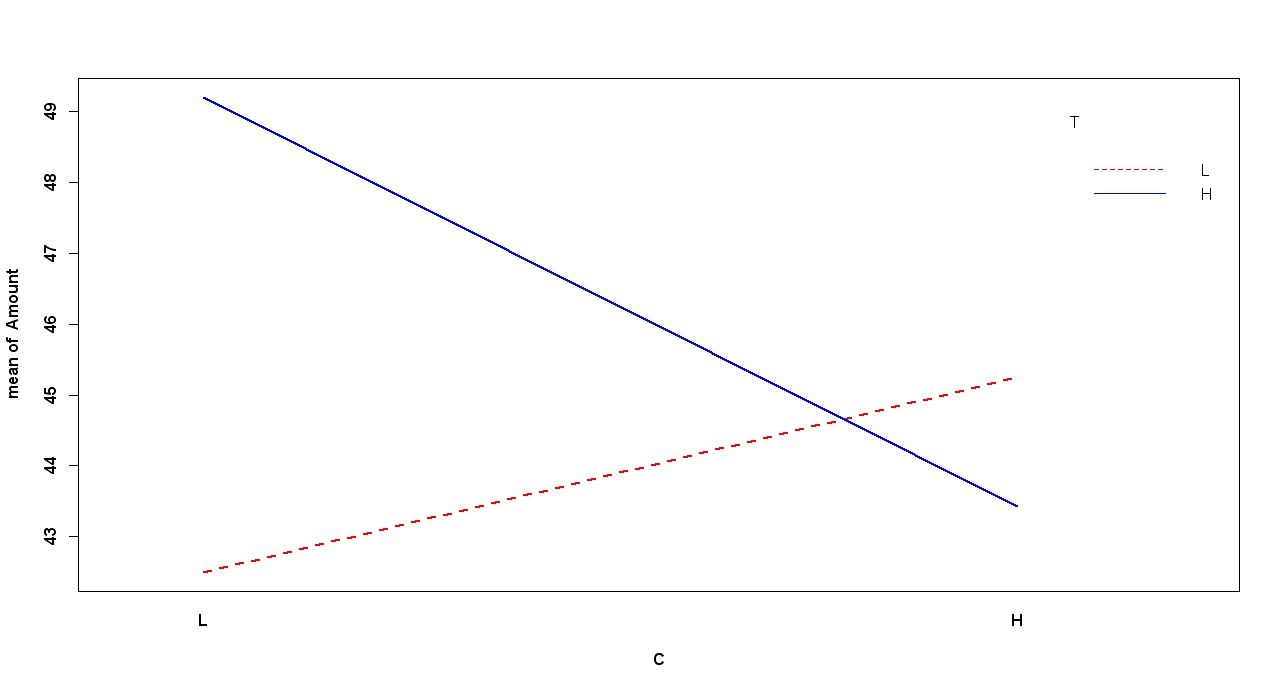
\includegraphics[scale=0.3]{images/ExamQ6interactionanew}
%\end{center}
%\begin{center}
%	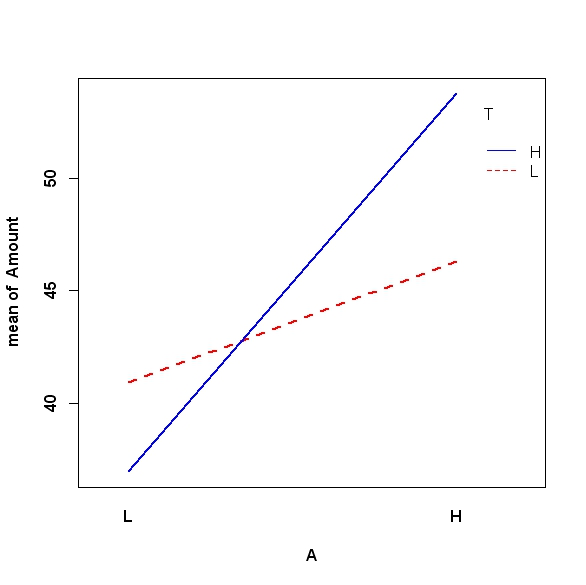
\includegraphics[scale=0.3]{images/ExamQ6interactionbnew}
%\end{center}
%\begin{center}
%	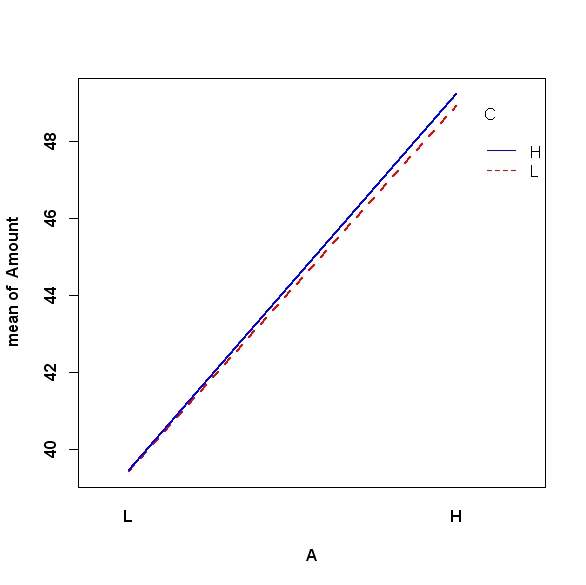
\includegraphics[scale=0.3]{images/ExamQ6interactioncnew}
%\end{center}

%================================================================ %
\newpage

\subsection*{Question 37} Six analysts each made seven determinations of the paracetamol content of the same batch of tablets.
The results are shown below. There are 42 determinations in total. The mean determination for each analysts is also tabulated. \\


%Analyst= structure(c(1L, 2L, 3L, 4L, 5L, 6L, 1L, 2L, 3L, 4L, 5L, 6L, 1L,
%2L, 3L, 4L, 5L, 6L, 1L, 2L, 3L, 4L, 5L, 6L, 1L, 2L, 3L, 4L, 5L,
%6L, 1L, 2L, 3L, 4L, 5L, 6L, 1L, 2L, 3L, 4L, 5L, 6L), .Label = c("A",
%"B", "C", "D", "E", "F"), class = "factor")

%Determinations= c(84.32, 84.24, 84.29, 84.14, 84.5, 84.7, 84.61, 84.13, 84.28,
%84.48, 83.91, 84.36, 84.64, 84, 84.4, 84.27, 84.11, 84.61, 84.62,
%84.02, 84.63, 84.22, 83.99, 84.15, 84.51, 84.25, 84.4, 84.22,
%83.88, 84.17, 84.63, 84.41, 84.68, 84.02, 84.49, 84.11, 84.51,
%84.3, 84.36, 84.33, 84.06, 83.81)

\begin{center}
	\begin{tabular}{|c|ccccccc|}
		\hline
		Analyst	& Content		&		&		&		&		&		&		 \\ \hline
		A	&	84.32	&	84.61	&	84.64	&	84.62	&	84.51	&	84.63	&	84.51	 \\
		B	&	84.24	&	84.13	&	84.00	&	84.02	&	84.25	&	84.41	&	84.30	 \\
		C	&	84.29	&	84.28	&	84.40	&	84.63	&	84.40	&	84.68	&	84.36	 \\
		D	&	84.14	&	84.48	&	84.27	&	84.22	&	84.22	&	84.02	&	84.33	 \\
		E	&	84.50	&	83.91	&	84.11	&	83.99	&	83.88	&	84.49	&	84.06	 \\
		F	&	84.70	&	84.36	&	84.61	&	84.15	&	84.17	&	84.11	&	83.81	 \\
		\hline
	\end{tabular}
\end{center}
\bigskip
The following \texttt{R} output has been produced as a result of analysis of these data:

%Experiment=data.frame(Determinations, Analyst)
%Model=aov(Determinations~Analyst)
%summary(Model)

%Analysis of Variance Table
%
%            Df Sum Sq Mean Sq F value  Pr(>F)
%Analyst      5 0.8611 0.17222   4.236 0.00394 **
%Residuals   36 1.4635 0.04065
%---
%Signif. codes:  0 ‘***’ 0.001 ‘**’ 0.01 ‘*’ 0.05 ‘.’ 0.1 ‘ ’ 1

\begin{center}
	\texttt{
		\begin{tabular}{|c|cccccc|}
			\hline
			% after \\: \hline or \cline{col1-col2} \cline{col3-col4} ...
			&&		&		&		&		&		\\
			Response: Y        	&&	Df  	&	Sum Sq 	&	Mean Sq 	&	F value    	&	$Pr(>F)$    	\\
			&&		&		&		&		&		\\\hline
			&&		&		&		&		&		\\
			Analyst 	&&	\textbf{?}	&	\textbf{?}	&	\textbf{?}	&	\textbf{?}	&	0.00394 **	\\
			&&		&		&		&		&		\\ \hline
			&&		&		&		&		&		\\
			Residuals	&&	\textbf{?}	&	\textbf{?}	&	0.04065	&	&		\\
			&&		&		&		&		&		\\ \hline
			&&		&		&		&		&		\\
			Total	&&	\textbf{?}	&	2.3246	&		&		&		\\
			&&		&		&		&		&		\\ \hline
		\end{tabular}
	}
\end{center}
\begin{itemize}
	\item[i.] (5 marks) Complete the ANOVA table in your answer sheet, replacing the "?" entries with the correct values.
	\item[ii.] (2 marks) What hypothesis is being considered by this procedure.
	\item[iii.] (2 marks) What is the conclusion following from the above analysis? State the null and alternative hypothesis clearly.
\end{itemize}
\newpage


\subsection*{Question 38 - Assumptions for ANOVA}

The \texttt{R} code and graphical procedures, below and on the following page, are relevant to checking whether the underlying assumptions are met for the ANOVA model in part (b).
\begin{itemize}
	\item[i.] (3 marks) What are the assumptions underlying ANOVA?
	\item[ii.] (4 marks)  Assess the validity of these assumptions for the ANOVA model in the previous question (Question 37).
	
\end{itemize}
\begin{framed}
	\begin{verbatim}
	Shapiro-Wilk normality test
	
	data:  Residuals
	W = 0.9719, p-value = 0.3819
	\end{verbatim}
\end{framed}
\begin{framed}
	\begin{verbatim}
	Bartlett test of homogeneity of variances
	
	data:  Experiment
	Bartlett's K-squared = 105.9585, df = 1, p-value < 2.2e-16
	\end{verbatim}
\end{framed}
\begin{center}
	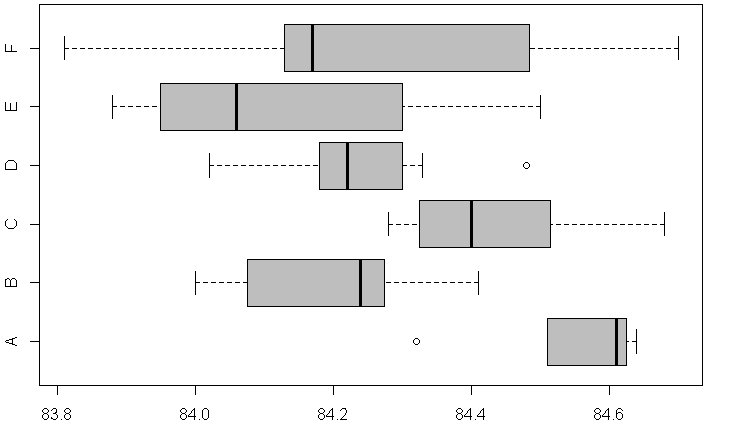
\includegraphics[scale=0.59]{images/ExamQ5boxplot}
\end{center}
\newpage
%qqnorm(resid(Model),pch=18,col="red",font.lab=2,font.axis=2)
%qqline(resid(Model))
\begin{center}
	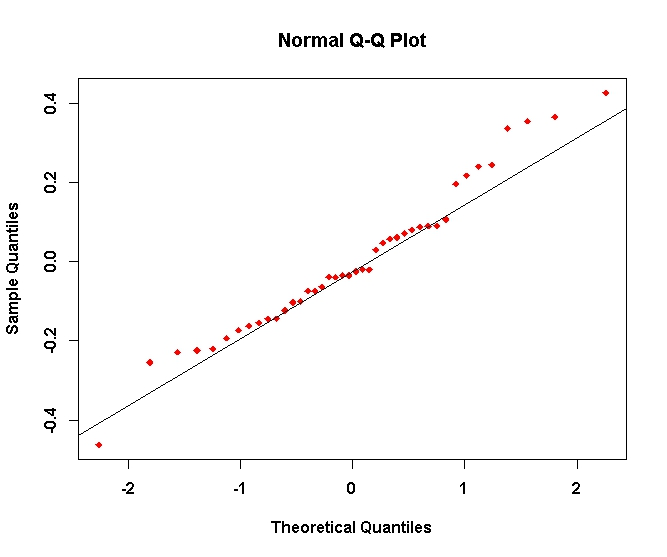
\includegraphics[scale=0.55]{images/ExamQ5qqplot}
\end{center}
\begin{center}
	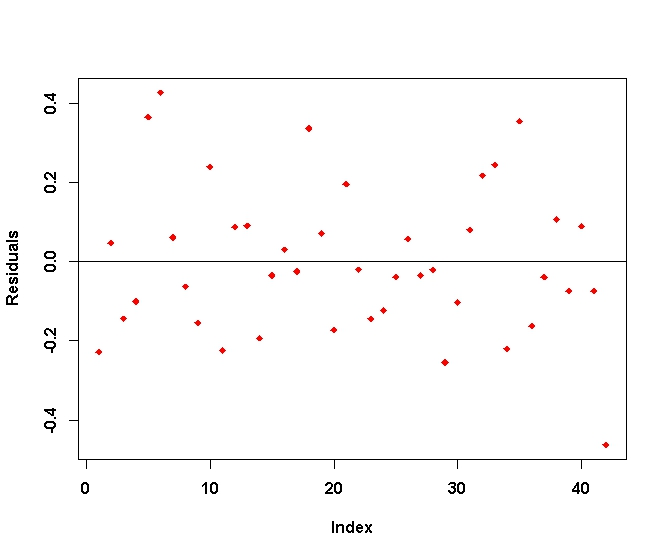
\includegraphics[scale=0.55]{images/ExamQ5resid}
\end{center}
\newpage



\subsection*{Question 39 - Control Charts Arithmetic}
A normally distributed quality characteristic is monitored through the use of control charts. These charts have the following parameters. All charts are in control.
	\begin{center}
		\begin{tabular}{|c|c|c|c|}
			\hline  & LCL & Centre Line & UCL \\
			\hline $\bar{X}$-Chart & 614 & 620 & 626 \\
			\hline $R$-Chart & 0 & 8.236 & 18.795 \\ \hline
		\end{tabular}
	\end{center}
	
	\begin{itemize}
		\item[i.] (2 marks) What sample size is being used for this analysis?
		\item[ii.] (2 marks) Estimate the standard deviation of this process.
		\item[iii.] (2 marks) Compute the control limits for the process standard deviation chart (i.e. the s-chart).
	\end{itemize}
	
\subsection*{Question 40 - Process Capability Indices}

An automobile assembly plant concerned about quality improvement measured sets of five camshafts on twenty occasions throughout the day. The specifications for the process state that the design specification limits at 600$\pm$3mm.
	
	
	\begin{itemize}
		\item[i.] (2 marks) Determine the \emph{Process Capability Indices} $C_p$ and $C_{pk}$, commenting on the respective values. You may use the \texttt{R} code output on the following page.
		\item[ii.] (2 marks)  The value of $C_{pm}$ is $1.353$. Explain why there would be a discrepancy between $C_p$ and $C_{pm}$.
		\item[iii.] (2 marks) Comment on the graphical output of the \emph{Process Capability Analysis}, also presented on the next page.
	\end{itemize}
	
	
	\newpage
	\begin{framed}
		\begin{verbatim}
		Process Capability Analysis
		
		Call:
		process.capability(object = obj, spec.limits = c(597, 603))
		Number of obs = 100          Target = 600
		Center = 599.548         LSL = 597
		StdDev = 0.5846948       USL = 603
		
		Capability indices:
		Value   2.5%  97.5%
		Cp    ...
		Cp_l  ...
		Cp_u  ...
		Cp_k  ...
		Cpm   1.353  1.134  1.572
		Exp<LSL 0%   Obs<LSL 0%
		\end{verbatim}
	\end{framed}
	
	
	
	\begin{center}
		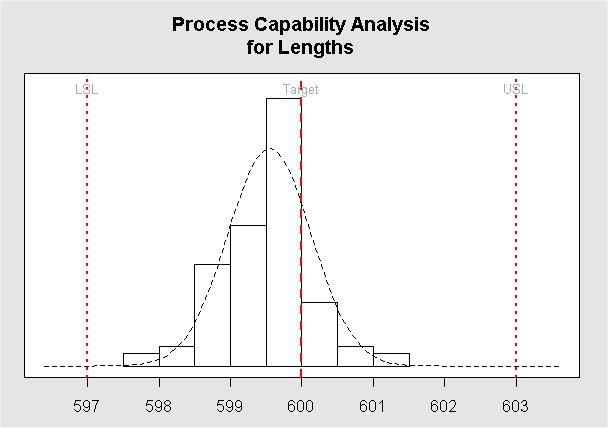
\includegraphics[scale=0.55]{images/ExamQ4hist}
	\end{center}
	\newpage
	%
	%Lengths = Values
	%
	%obj <- qcc(Lengths, type="xbar")
	%
	%process.capability(obj, spec.limits=c(597,603))

\subsection*{Question 41}
Answer the following questions.

\begin{itemize}
	\item[i] (1 marks) Differentiate common causes of variation in the quality of process output from assignable causes.
	\item[ii.] (1 marks) What is tampering in the context of statistical process control?
	\item[iii] (4 marks) Other than applying the \emph{Three Sigma} rule for detecting the presence of an assignable cause, what else do we look for when studying a control chart? Support your answer with sketches.
\end{itemize}

\subsection*{Question 42- Control Charts Arithmetic}

A normally distributed quality characteristic is monitored through the use of control charts. These charts have the following parameters. All charts are in control.
\begin{center}
	\begin{tabular}{|c|c|c|c|}
		\hline  & LCL & Centre Line & UCL \\
		\hline $\bar{X}$-Chart & 542 & 550 & 558 \\
		\hline $R$-Chart & 0 & 8.236 & 16.504 \\ \hline
	\end{tabular}
\end{center}

\begin{itemize}
	\item[i] (2 marks) What sample size is being used for this analysis?
	\item[ii.] (2 marks) Estimate the standard deviation of this process.
	\item[iii.] (2 marks) Compute the control limits for the process standard deviation chart (i.e. the s-chart).
\end{itemize}

\subsection*{Question 43 - Process Capability Indices} 

An automobile assembly plant concerned about quality improvement measured sets of five camshafts on twenty occasions throughout the day. The specifications for the process state that the design specification limits at 600$\pm$3mm.


\begin{itemize}
	\item[i.] (4 marks) Determine the \emph{Process Capability Indices} $C_p$ and $C_{pk}$, commenting on the respective values. You may use the \texttt{R} code output on the following page.
	\item[ii.] (2 marks)  The value of $C_{pm}$ is $1.353$. Explain why there would be a discrepancy between $C_p$ and $C_{pm}$.
	\item[iii.] (2 marks) Comment on the graphical output of the \emph{Process Capability Analysis}, also presented on the next page.
\end{itemize}


\newpage
\begin{framed}
	\begin{verbatim}
	Process Capability Analysis
	
	Call:
	process.capability(object = obj, spec.limits = c(597, 603))
	Number of obs = 100          Target = 600
	Center = 599.548         LSL = 597
	StdDev = 0.5846948       USL = 603
	
	Capability indices:
	Value   2.5%  97.5%
	Cp    ...
	Cp_l  ...
	Cp_u  ...
	Cp_k  ...
	Cpm   1.353  1.134  1.572
	Exp<LSL 0%   Obs<LSL 0%
	\end{verbatim}
\end{framed}



\begin{center}
	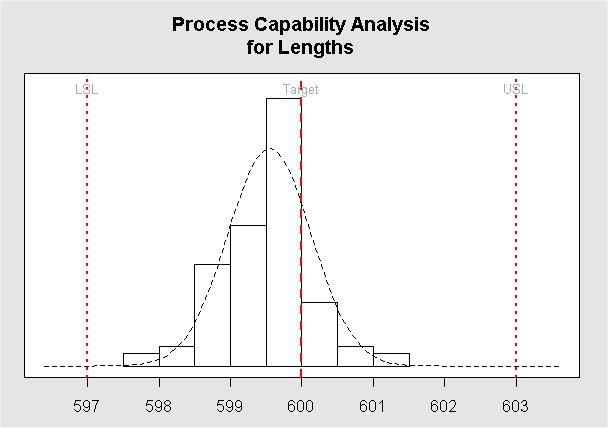
\includegraphics[scale=0.55]{images/ExamQ4hist}
\end{center}
\newpage
%
%Lengths = Values
%
%obj <- qcc(Lengths, type="xbar")
%
%process.capability(obj, spec.limits=c(597,603))
\subsection*{Question 44}
An experiment is run on an operating chemical process in which the aim is to reduce the
amount of impurity produced. Three continuous variables are thought to affect impurity,
these are concentration of NaOH, agitation speed and temperature. As an initial investigation two settings are selected for each variable these are

\begin{center}
	\begin{tabular}{|c|c|c|}
		\hline
		% after \\: \hline or \cline{col1-col2} \cline{col3-col4} ...
		Factor: &low level & highlevel  \\ \hline
		Concentration of NaOH & $40\%$ & $45\%$\\
		Agitation speed (rpm) & 15 & 25 \\
		Temperature ($^{\circ}{\rm F}$) & 170 & 200 \\
		\hline
	\end{tabular}
\end{center}
Readings were recorded of the impurity produced from the chemical process for each combination of the levels of these factors, and each combination was tested twice.
\begin{center}
	\begin{tabular}{|c|c|c|c|}
		\hline
		% after \\: \hline or \cline{col1-col2} \cline{col3-col4} ...
		Conc NaOH & Agitation & Temperature & Impurity \\
		-	&	-	&	-	&	 90,70	\\
		+	&	-	&	-	&    100,120	\\
		-	&	+	&	-	&	 90,110	\\
		+	&	+	&	-	&	 120,150	\\
		-	&	-	&	+	&	 110,100\\
		+	&	-	&	+	&	 100,130	\\
		-	&	+	&	+	&	 100,80	\\
		+	&	+	&	+	&	 160,140\\
		\hline
	\end{tabular}
\end{center}
\begin{itemize}
	\item[i.] (8 Marks) Calculate the contrasts, the effects and the sum of squares for the effects.
	\item[ii.] (8 Marks) Using the computed sums of squares values, complete the ANOVA table (see the \texttt{R} code below).
	\item[iii.] (4 Marks) Comment on the tests for significant for the main effects and interactions. State clearly your conclusions.
	\item[iv.] (4 Marks) Write down a  regression equation that can be used predicting impurity based on the results of this experiment.
\end{itemize}

\begin{framed}
	\begin{verbatim}
	Df Sum Sq Mean Sq F value  Pr(>F)
	Conc            1    ...     ...   ...   0.00253 **
	Agit            1    ...     ...   ...   0.07093 .
	Temp            1    ...     ...   ...   0.29485
	Conc:Agit       1    ...     ...   ...   0.48239
	Conc:Temp       1    ...     ...   ...   0.87675
	Agit:Temp       1    ...     ...   ...   0.44646
	Conc:Agit:Temp  1    ...     ...   ...   0.18751
	Residuals       8   1950     244
	\end{verbatim}
\end{framed}

\newpage
\begin{center}
	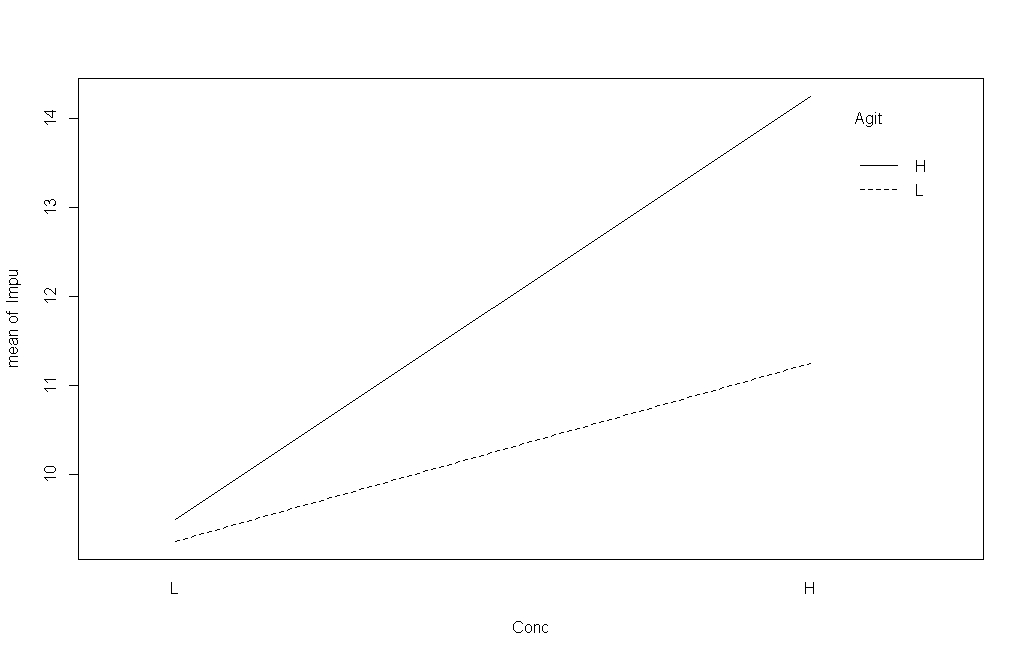
\includegraphics[scale=0.3]{image/ExamQ6interactiona}
\end{center}
\begin{center}
	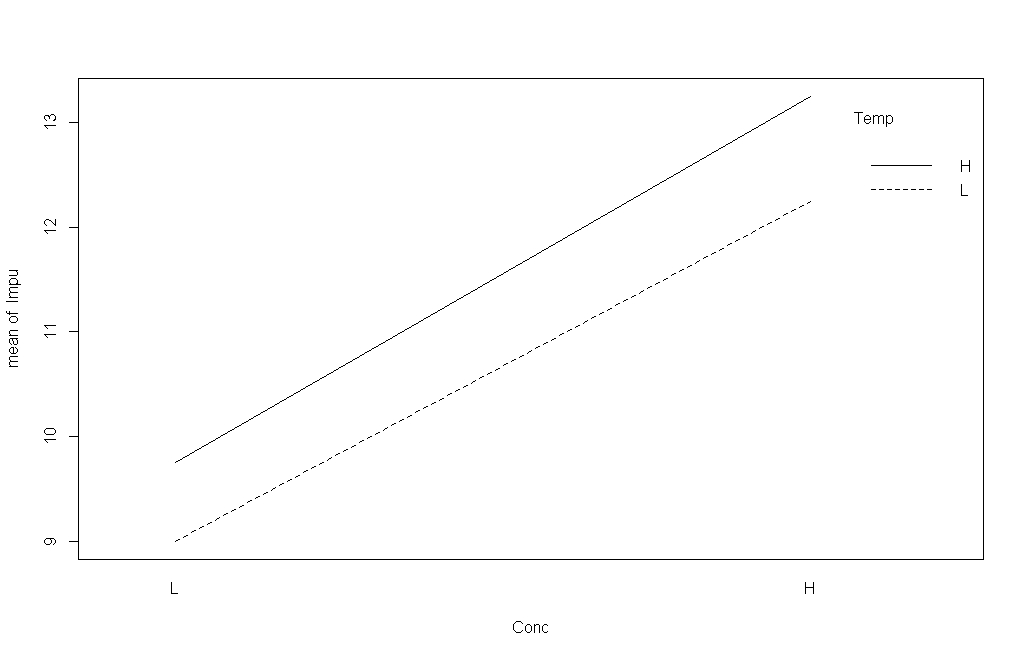
\includegraphics[scale=0.3]{image/ExamQ6interactionb}
\end{center}
\begin{center}
	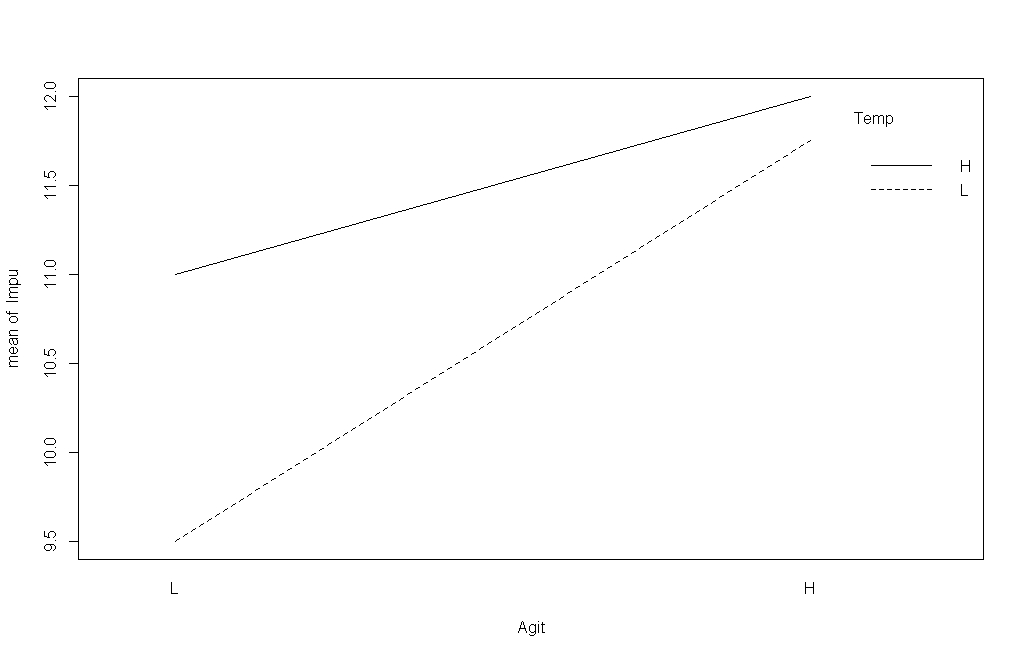
\includegraphics[scale=0.3]{image/ExamQ6interactionc}
\end{center}

\newpage
\subsection*{Question 45}
Answer the following questions.

\begin{itemize}
	\item[i.] (1 marks) What is the purpose of maintaining control charts?
	\item[ii.] (1 marks) What is the \emph{Three Sigma} rule in the context of statistical process control?
	\item[iii.] (4 marks) Other than applying the \emph{Three Sigma} rule for detecting the presence of an assignable cause, what else do we look for when studying a control chart? Limit your answer to three examples. Support your answer with sketches.
	\item[iv.] (2 Marks) What is a CUSUM chart? What type of departures from the production target value
	is this type of chart useful for detecting?
\end{itemize}
\end{document}